\documentclass[a4paper,12pt]{report}
\author{}
\date{}

\usepackage[shortlabels]{enumitem}
\usepackage{graphicx}
\usepackage{hyperref}
\usepackage{varioref}

% \usepackage{verbatim}
% \newcommand{\detailtexcount}[1]{%
% \immediate\write18{texcount -merge -sum -q #1.tex references.bib > #1.wcdetail }%
% \verbatiminput{#1.wcdetail}%
% }

\graphicspath{ {./images/} }
\hypersetup{
    colorlinks=true,
    linkcolor=blue,
    filecolor=magenta,      
    urlcolor=cyan,
    pdfpagemode=FullScreen,
    }

\begin{document}
    \begin{titlepage}
        \begin{center}
            
            \textbf{\Large Application of AI on IT Service Management}
                
            \vspace{1.5cm}

            \begin{figure}[h]
                
\includegraphics[scale=1.0]{EPITA.jpg}
                \centering
            \end{figure}
    
            \begin{center}
                \centerline{Arun Singh SIVAPRAKASH}
                \centerline{Pramod Kumar NAGARAJ}
                \centerline{Van Tien NGUYEN}
                \centerline{Alexander POPPE}
            \end{center}
    
            \vfill

            \centerline{EPITA Graduate School of Computer Science}
            
                
            \begin{center}
                \centerline{Advisor}
                \centerline{ Olivier BERTHET}
            \end{center}
        
            \begin{center}
                Master of Science in Artificial Intelligence Systems
            \end{center}
        
            \vfill
            \centerline{16-07-2021}
                
        \end{center}
    \end{titlepage}


    \setcounter{page}{1}
    \small\tableofcontents

    
    % \pagebreak
    % \detailtexcount{Thesis}

    \begin{abstract}
        Large enterprise Information technology infrastructure components generate large volume of alerts and incident tickets. These are manually screened, but it is otherwise difficult to extract information automatically from them to gain insight in order to improve operational efficiency. We propose a framework to cluster alters and incident tickets based on the text in them, using unsupervised machine learning. This would be a step towards eliminating manual classification of the alters and incidents, which is very labour intense and costly.
        \newline\newline
        The challenges that arrive at analysing huge amount text data starts with the data quality. Data quality metrics concerning the interpretation of text are too difficult to compute automatically and too pragmatic because they heavily depend on the linguistic content and the specific situation in which the text is being used. Several statistical approaches have been used to determine some level of data quality in this project.   
        \newline\newline
        The visual representation of text data helps to bring more insights from the data. Building dashboard with various filters will help the users to customize the search. We have implemented state of art visualization dashboards with different open-source tools.
        \newline\newline
        We proposed the techniques to visualize the clusters that make human readable in an easy and understandable way compared to the traditional methods, we find a simple way to define prototype of cluster for easy interpretation. This framework for clustering and visualization will enable enterprises to prioritize the issue in their IT infrastructure and improve the reliability and availability of their services.
    \end{abstract}

    \chapter{Introduction}
    \section{Motivations}
    Organization of all sizes struggles with a common problem in Infrastructure and Operational Management. Thousands of automated alerts with semi- structure text are generated every day from hundreds of infrastructure tools. There are thousands of incidents tickets with manually entered unstructured text are created daily by support personnel. After collecting all the details of the incidents maintaining of those tickets is very hard and costly and difficult to analysis each incident without grouping them. This is not only a frustrating situation for the company but also for clients. 
    \newline\newline
    Many of us have been forced to take time out of our schedule to e-mail or call a helpdesk with an IT related question. Redirection of the calls in order to get the right person on the line is not very rare. This can cause some frustration and time which is not beneficial for both parties. 
    \newline\newline
    IT problems exist and they will always exist. We can try to prevent them as much as possible but that is not the only solution. Dealing with them in an appropriate and efficient manner is the goal of this research. By looking into the similarity between tickets, tickets can be directly assigned to a dedicated team. This should improve the efficiency and reduce any unnecessary redirection. This research also looks into the quality of a ticket. This provides more insight in how problems are documented and where to improve the service. A good documentation of a problem will always help to find a solution. 



    \section{Context of the Project}
    Organization operating in IT enables business segment over a decade. On an average, the company receives more than 25k IT incidence or tickets. Which are handled to best practice by certain framework which are done by researchers with incident management, problem management etc. 
    \newline\newline
    We are developing the framework which help the IT tech companies to visualize the data quality and data clustering. With this, the company can understand the problem of the user in systematic manner within no time, and the companies  auto robots can answer for the user  problem with more effectively.
    
    \section{Objectives and Contributions}
    Objective of this project is to provide the enterprise various tools and mediums that leverages the latest State of Art NLP and machine learning techniques to 
    analyse their incident management system. These tools will bring out the hidden insights in the ticket data which will enable the users to take data driven decisions for the business improvements.
    \newline\newline
    Data quality of the raw text data has been identified with statistical tests.
    Insight’s dashboard can help the company to improve the performance of the service teams and to track which sections need more attention. This will also help in the resource allocation among various sections and also in effective cost management. Clustering application will bring out the similar ticket records based on the input description, this will help the teams to get the details of tickets which were similar to the entered description and how they were resolved before. This will help in reducing time ticket resolve time.


    
    \section{Overview of thesis}
    In this thesis we have implemented various ML and NLP techniques to generate the business insights from the raw text data. We discussed in detail about the clustering of similar tickets and its implementation using various technologies in real time.

    \chapter{State of Art}
    Natural language processing (NLP)\cite{NLPWiki} is a subfield of linguistics, computer science, and artificial intelligence concerned with the interactions between computers and human language, in particular how to program computers to process and analyze large amounts of natural language data. The goal is a computer capable of "understanding" the contents of documents, including the contextual nuances of the language within them. The technology can then accurately extract information and insights contained in the documents as well as categorize and organize the documents themselves.
    In our project, NLP is used to extract information tickets and evaluate the quality of data.

    \section{NLP pipeline}
    In general, NLP contains three main stages: text processing, feature extraction, modeling\cite{IntroNLP}.
    \begin{figure}[!h]
        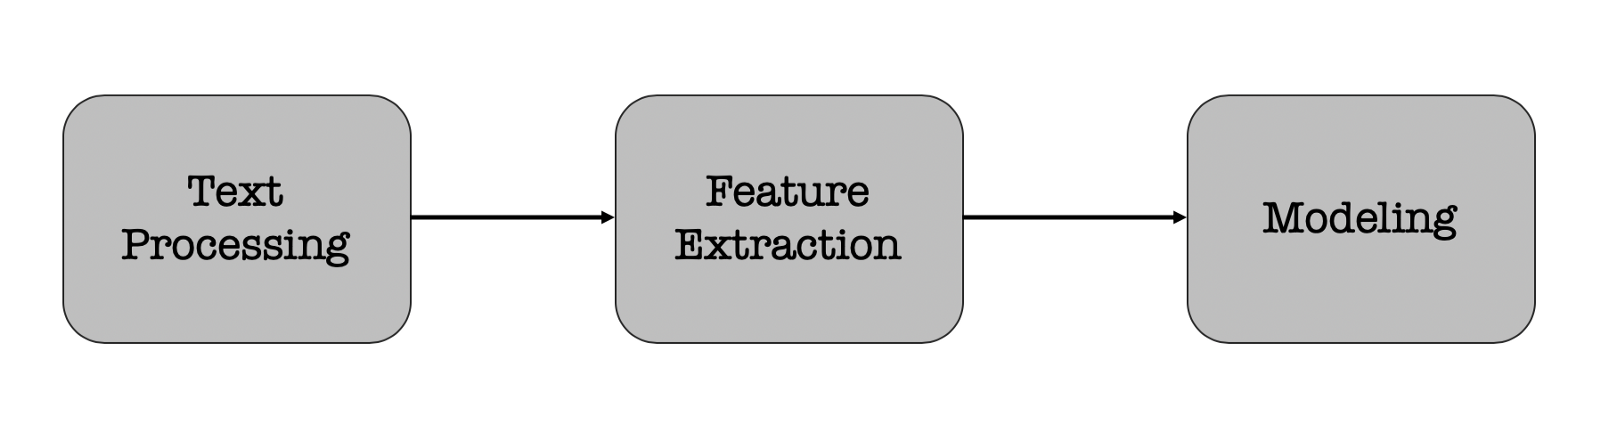
\includegraphics[width=\linewidth]{nlp_pipeline.png}
        \centering
        \caption{NLP pipeline}
    \end{figure}

    \subsection{Text Processing}
    In this step, we take text raw as an input. Then we process the input into a form that is the best for next step: feature extraction.
    More specifically, raw data needs to be cleaned that means removing special characters such as HTML tags, etc. In other words, input data does not contain any info for the model to lean and are irrelevant or noisy data.
    After that, we do the data normalization which involes the case normalization, punctuation removal so that the text is in a single format for the machine to learn.
    In case normalization, we convert all capitalization to lower to bring a common case, 
    and in punctuation removal, we replace all punctuations with space.
    The next process is breaking up text documents into individual words called tokens and remove the stop words.
    Stop word removal means removing the non-important words like "a", "is", "the", "and", "an", etc. 
    \newline\newline
    After that, we need to reduce words to its normalized form, and this process can be done by stemming or lemmatization technique.
    Stemming is a process of reducing a word to its root form, for example: "branching", "branched" and "branches" can all be reduced to "branch", 
    meanwhile lemmatization is the algorithmic process of determining the canonical
    form (lemma) of a word.
    Unlike stemming, it is not only a word reduction but depends on the
    meaning of the word in a sentence and needs to consider a language’s
    full vocabulary, for instance: "was" will be transformed into "be", "meeting" will be "meet" or "meeting" depending on the context.

    \subsection{Feature Extraction}
    Feature Extraction is a way of extracting feature vectors from the text after the text processing step so that it can be used in the machine learning model as input.
    Word Embedding is one such technique where we can represent the text using vectors. The more popular forms of word embeddings are:
    Bag-of-Words (BoW) and Term Frequency-Inverse Document Frequency (TF-IDF).
    \newline\newline
    Bow is a way of extracting features from the text for use in modeling, it treats each document as a collection or bag of word. This means a representation of text that describes the occurrence of words within a document.
    It involes two things: a vocabulary of known words in the corpus (set of documents) and a measure of the presence of known words.
    Term Frequency-Inverse Document Frequency is a ponderation method uused in information retrieval. This statistical measure gives an evaluation of how important is a word to a document, depending on the corpus considered.
    TF-IDF is calculated as: $tfidf(t,d,D) = tf(t,d) * idf(t,D)$.
    Inverse document frequency:
    \begin{math}
        idf(t,D) = \log(\frac{N}{|\{d\in D:t\in d\}|})
    \end{math}
    with N the number of documents in corpus D.
    \newline\newline
    For example: we have two documents which are Document1 "Xavier likes to play football. Eric likes football too." and Document2 "Eric prefers tennis to football", we can have the representation below:
    \begin{figure}[!h]
        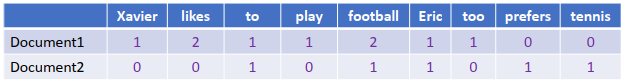
\includegraphics[width=\linewidth]{bow.png}
        \centering
        \caption{Example of BoW}
    \end{figure}

    \begin{figure}[!h]
        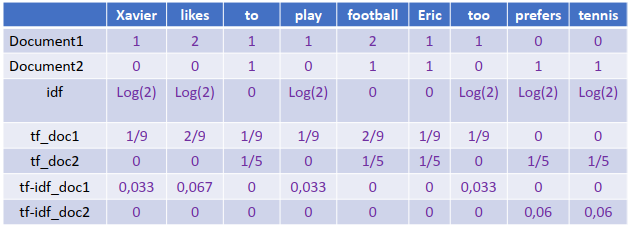
\includegraphics[width=\linewidth]{tf-idf.png}
        \centering
        \caption{Example of TF-IDF calculation}
    \end{figure}

    \subsection{Modeling}
    The final stage of the NLP pipeline is modeling, which includes designing a statistical or machine learning model, 
    fitting its parameters to training data, using an optimization procedure, and then using it to make predictions about unseen data.
    In our project, we use clustering machine learning algorithms.
    \newline\newline
    Clustering is an unsupervised machine learning task. It involves automatically discovering natural grouping in data. Unlike supervised learning, clustering algorithms only interpret the input data and find natural groups or clusters in features in feature space.
    A cluster is often an area of density in the feature space where examples from the domain (observations or rows of data) are closer to the cluster than other clusters. The cluster may have a center (the centroid) that is a sample or a point feature space and may have a boundary or extent.
    Clustering can be helpful as a data analysis activity in order to learn more about the problem domain. It also can be useful as a type of feature engineering, where existing and new examples can be mapped and labeled as belonging to one of the identified clusters in the data.
    \newline\newline
    Evaluation of identified clusters is subjective and my require a domain expert, although many clustering-specific quantitative measures do exist. Typically, clustering algorithms are compared academically on synthetic datasets with pre-defined clusters which an algorithm is expected to discover.
    There are two common clustering algorithms: K-Means and Gaussian Mixture Model.
    
    \subsubsection{K-Means:} 
    This is one of the simplest and frequently used unsupervised learning algorithms, especially in data mining and statistics. Being a portioning algorithm, its goal is to form groups of data points based on the number of clusters, represented by the variable k. K needs to be predefined before the execution. K-means uses an iterative refinement method to produce its final clustering based on the number of clusters defined by the user and the dataset. Initially, k-means randomly chooses k as the mean values of k clusters, called centroids, and find the nearest data points of the chosen centroids to form k clusters. Then, it iteratively recalculates the new centroids for each cluster until the algorithm converges to one optimum value. K-means clustering would be suited with the numerical data with a low dimensionality because numerical data is used to compute the mean value. The type of data best suited for K-means clustering would be numerical data with a relatively lower number of dimensions. 
    \newline\newline
    Problem description\cite{KMeanWiki}: A set of observations $(x_1, x_2, …, x_n)$ where each observation is a $d$-dimensional real vector, this algorithm aims to partition the n observations into $k(<=n)$ sets $S = \{S_1, S_2, …, S_k\}$ so as to minimize the within cluster sum of squares.
    \newline\newline
    Algorithm\cite{KMeanWiki}: initial randomly set of k means $(m_1, m_2, …, m_k$, the algorithm proceeds by altering between two steps.
    The first step is assignment step: assign each observation to the cluster with the nearest mean that with the least squared Euclidean distance:
    $S_i = \arg\min\limits_k||x_i - m_k||^2$. 
    The second step is update step which recalculates the means (centroids) for observation assigned to each cluster:
    $m_k = \frac{\Sigma_{i:k_i=k}x_i}{|i:k_i=k|}$.
    The algorithm has converged when the assignments no longer change.
    \newline\newline
    K-means has some advantages\cite{MinhLeKazuhiroOgata2019} which are simple clustering algorithm so that it can be implemeneted easily. It also faster computationally than other clustering algorithms because K-means has only a few comupations.
    Additionally, this algorithm can scale up to large dataset and easily adapt to new data samples.
    Besides, there are some disavantages: K-means has difficulty with clustering data set of varying sizes and density. Its result can also vary depending on inital values and the number is clusters has to be specified manually.    

    \subsubsection{Gaussian Mixture Model (GMM): }
    Probabilistic models and use the soft clustering approach for distributing the points in different clusters, it assumes that there are a certain number of Gaussian distributions and each of these distributions represent a cluster. therefore, a GMM tends to group the data points belonging to a single distribution together.
    \newline\newline
    Gaussian distribution (or Normal distribution)\cite{GMM}: is a type of continuous probability distribution for a real-valued random variable. The general form of its probability density function:
    $f(x) = \frac{1}{\sigma \sqrt{2\pi}}e^{-\frac{(x-\mu)^2}{2\sigma^2}}$, with parameters: $\mu$ is mean of the distribution and $\sigma$ is standard deviation.
    \newline\newline
    To implement GMM, we use Expectation-Maximization algorithm (EM)\cite{GMM}. EM is a statistical algorithm for finding the right model parameters.
    It typically used for handling missing values or in other words latent variables. This algorithm has two steps: E-step, the available data is used to estimate the values of the missing variables
    and M-step, based on the estimated values generated in the e-step, the complete data is used to update the parameters.
    \newline\newline
    EM in GMM\cite{GMM}: We need to assign k number of clusters. This means that there are k Gaussian distributions, with the mean and covariance values to be $\mu_1, \mu_2, ..., \mu_k$
    and $\sigma_1, sigma_2, ..., sigma_k$. Additionally, there is another parameter for the distribution that defines the number of points for the distribution. Or in other words, the density of the distribution is represented with $\Pi$


    \section{Text Data Visualization}
    Data visualization is essential to assist businesses in quickly identifying data trends, which would otherwise be a hassle. The pictorial representation of data sets allows analysts to visualize concepts and new patterns. With the increasing surge in data every day, making sense of the quintillion bytes of data is impossible without Data Proliferation, which includes data visualization.
    \newline\newline
    Every professional industry benefits from understanding their data, so data visualization \cite{DataVizImportance} is branching out to all fields where data exists. For every business, information is their most significant leverage. Through visualization, one can prolifically convey their points and take advantage of that information
    
    \subsection{Importance of Data Visualization}
    A dashboard, graph, infographics, map, chart, video, slide, etc. all these mediums can be used for visualizing and understanding data. Visualizing the data enable decision-makers to interrelate the data to find better insights and reap the importance of data visualization\cite{DataVizImportance}, which are:
    \subsubsection{Analysing the Data in a Better Way}
    Analysing reports helps business stakeholders focus on the areas that require attention. The visual mediums help analysts understand the key points needed for their business. Whether it is a sales report or a marketing strategy, a visual representation of data helps companies increase their profits through better analysis and better business decisions.
    \subsubsection{Faster Decision Making}
    Humans process visuals better than any tedious tabular forms or reports. If the data communicates well, decision-makers can quickly take action based on the new data insights, accelerating decision-making, and business growth simultaneously.
    \subsubsection{Making Sense of Complicated Data}
    Data visualization allows business users to gain insight into their vast amounts of data. It benefits them to recognize new patterns and errors in the data. Making sense of these patterns helps the users pay attention to areas that indicate red flags or progress. This process, in turn, drives the business ahead.

    \subsection{Tools used for Text Data Visualization}
    Data visualization tool provides users with an easier way to create visual representations of large data sets. When dealing with data sets that include hundreds of thousands or millions of data points, automating the process of creating a visualization, at least in part, makes a designer’s job significantly easier.
    \subsubsection{ELK STACK}
    The ELK\cite{ELK} stack is an acronym used to describe a stack that comprises of three popular open-source projects: Elasticsearch, Logstash, and Kibana. ELK stack gives us the ability to aggregate logs from all systems and applications, analyze these logs, and create visualizations for application and infrastructure monitoring, faster troubleshooting, security analytics, and more. 
    \newline\newline \textbf{E = Elasticsearch}
    \newline\newline
    Elasticsearch is an open-source, RESTful, distributed search and analytics engine built on Apache Lucene. Support for various languages, high performance, and schema-free JSON documents makes Elasticsearch an ideal choice for various log analytics and search use cases.
    \newline\newline \textbf{L = Logstash}
    \newline\newline
    Logstash is an open-source data ingestion tool that allows you to collect data from a variety of sources, transform it, and send it to your desired destination. With pre-built filters and support for over 200 plugins, Logstash allows users to easily ingest data regardless of the data source or type.
    \newline\newline \textbf{K = Kibana}
    \newline\newline
    Kibana is an open-source data visualization and exploration tool for reviewing logs and events. Kibana offers easy-to-use, interactive charts, pre-built aggregations and filters, and geospatial support and making it the preferred choice for visualizing data stored in Elasticsearch.
    \newline
    We have implemented the dashboard with ELK to visualize the ticket data and generate as much insights from it.


    \chapter{System's Architecture}\label{SystemArchitechture}
    \section{Insights Dashboard Architecture}
    Raw Text data can be sent into ELK through Elasticsearch or Logstash. Logstash parses and the transforms the data and push it into Elasticsearch where the data is indexed. Kibana is used to create charts, graphs and dashboards. ELK is scalable and easier to deploy in both cloud and on-premise architecture. Below is the pictorial representation of implementation.
    \newline\newline
    \begin{figure}[!h]
        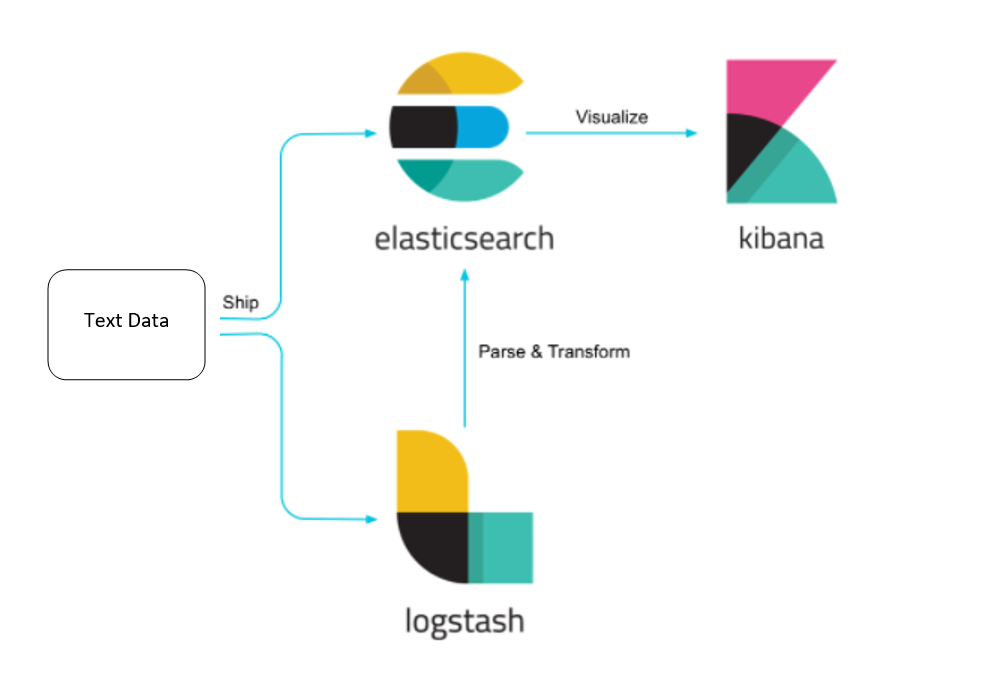
\includegraphics[scale=0.5]{dashboard.png}
        \centering
        \caption{Dashboard Artchitecture}
    \end{figure}
    
    \section{Clustering System Artchitecture}
    We processed to have a system architecture which is built on the streamlit and FASTAPI framework. We will make use of different tools to build our web application for IT ticket clustering.
    \newline\newline
    Initially, we select the raw data given by the company. We do data pre-processing and this data will be sent to model either KNN or GMM. The model is trained with the pre-processed data. Later, the trained model is called through FASTAPI and post the request to streamlit as a frontend.
    After deploying the application, the user will be able to rise his incidence ticket and the data will be pre-processed and the model will use this pre-processed text to cluster similar tickets and return the output to frontend.
    \newline\newline
    \begin{figure}[!h]
        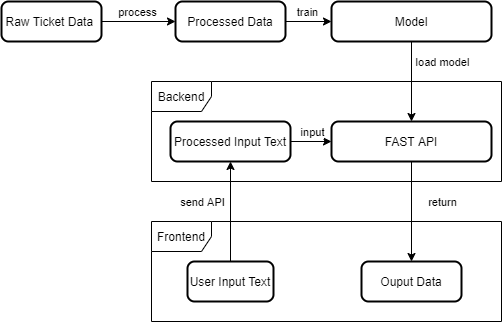
\includegraphics[width=\linewidth]{System's Artchitecture.png}
        \centering
        \caption{Clustering System Artchitecture}
    \end{figure}
    
    \chapter{Methodology}
    \section{Data Visualization – ELK Dashboard}

    We have implemented our visualization architecture in a Ubuntu Machine. Single-Node ELK Stack\cite{ELKLog} is installed in Ubuntu 20.04. Our text data is fairy small and we are not connected into a live stream of tickets. Hence Single Node ELK Stack is sufficient of our analysis. Data is sent into ELK through Logstash, indexed in elastic search and visualized in KIBANA. Custom filters are created that enables the users to make advanced searches and find insights. 
    \newline
    Dash Board can be shared to anyone in the organization’s WLAN and also can be hosted online. But accruing SSH certificates and domain registration are beyond the scope of this project.


    \section{Clustering}
    \begin{figure}[!h]
        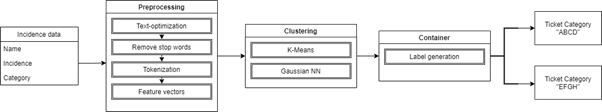
\includegraphics[width=\linewidth]{clustering_motho.png}
        \centering
        \caption{Clustering Pipeline}
    \end{figure}
    
    \noindent In order to categorize incident tickets, the tickets are pre-processed and converted into feature vectors, and cluster algorithms are applied for categorizations. In the last step, the incidence is meaningfully assigned to a specific category. After initial clustering, the trained algorithm can be saved to get fixed categories and to predict the category of new incidence tickets later. Now we can read about each component in details.
    \section{Data exploratory}
    In order to have a better understanding of the data collected and integrated for clustering, we performed extensive exploratory data analysis on various features of the data. This step is highly significant in helping us to understand the distribution of target fields and different categories. After pre-processing, we removed the words which had no information using NLTK framework and extract feature vector.

    \section{Algorithm}
    \subsection{K-Means}
    We use K-means because it is a simple baseline algorithm. K-means represent a simple algorithm to classify data into cluster. K-means works in three steps, first it will initiate the random cluster centroids. Second, each data point is assigned to the cluster with the smallest distance. On the last step, the steps 2 are repeated until the cluster centroids unchanged.

    \subsection{Gaussian Mixture Model}
    We use Gaussian mixture model because it presents a powerful tool for clustering. It assumes that each data group can be reasonably described by one mixture model component. This establishes a one-to-one relationship between mixture component and cluster. The idea for using this algorithm to alleviate the error occurs due to collection of records in different ways and give more efficient results. The working of this model is explained in the state of the art.

    \section{Label generation}
    Without descriptive cluster names, it is difficult for a human to gather information from the grouped document. Getting the understandable description to human is the most difficultly task. For the algorithm form the field of supervised learning, this is easily possible to form the training data. However, those are not present during clustering. The Cluster labelling is done in many ways. The most popular methods are human labelling, automatic labelling, and semi-automatic labelling. In the human labelling, it's manually labelling the cluster by humans how creates a name after visual inspection of same documents of cluster. Automatic methods is to generate the cluster names from most powerful features within a cluster. Semi-clustering means customizing the automatic cluster names by humans or list of cluster names predefined, subsequently the documents are automatically sorted into categorize. For K-means algorithm, the information can be obtained from the cluster centroids. The cluster centroids are located in the features space and therefore have the same dimension as the tf-idf feature vectors. In order to obtain a list of words sorted by relevance for K-means, the values of cluster centroids must be sorted.
    
    \chapter{Results}
    This document is made in preparation of the actual Action week where our main focus will be the coding and producing actual results. During this preparation and literature review, we are not producing definite results yet. However, we have an idea about what might be possible, and which results previous work yielded. For this chapter, the basis will be previous work and results that they obtained. This will be our goal for next week to reach. We should find adapt existing research to our problem at hand and try to also provide accurate result for this use case.
    \newline\newline
    There has been a lot of research that studies the similarity between tickets. This gives us some interesting information which can be adapted to our use case. At the moment, ServiceNow is a service that is often used to process tickets. Although they are providing a good service, some improvements can be made. Article\cite{Garrett2020} explores an alternative model to what ServiceNow is providing. They improve the accuracy of ServiceNow from 40\% to 85\%. This is a very significant improvement and also something we should be aiming for during the implementation of our model.

    \section{Development Anticipated}
    We have planned perform several statistical tests to analyse the quality of the text data.
    As a part of insights generation from data we have planned to implement a dashboard with ELK stack. In Clustering Application, we intent to group the cluster the tickets and build a model that can interact with the Streamlit UI and FastAPI to return details of the similar tickets.

    
    \chapter{Conclusion}
    In this paper, we explained the background of our challenge which is the need for an improved IT System Management (ITSM). This includes two main parts, mapping similarity between tickets and visualising the quality of a ticket. In our literature review, we found state-of-the-art implementations of ITSM and NLP implementations that can help us to reach our goal. The remaining time of this project, we will focus on the coding part and adapting all research to our specific use case. The key in this research is to present our results with to-the-point visualisations for which we will use a dashboard as described in chapter \vref{SystemArchitechture}.

    
    \nocite{*}

    \bibliographystyle{IEEEtran}
    \bibliography{references.bib}

    
    \listoffigures
    
    \newpage
    \begin{figure}[!h]
        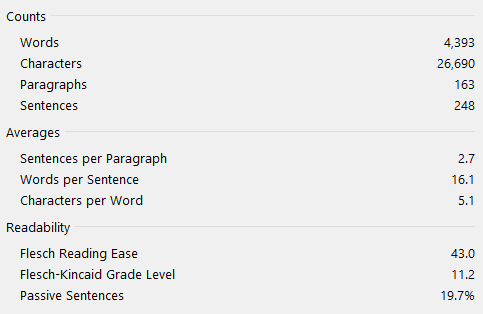
\includegraphics[width=\linewidth]{readability.png}
        \centering
        \caption{Readability Statistics}
    \end{figure}

\end{document}